
\documentclass[refcompress,eversion,noinfo]{BESTIthesis}
\usepackage{multirow}
\usepackage{graphicx}
\usepackage{diagbox}
\usepackage[subrefformat=parens,labelformat=parens]{subfig}
\usepackage{caption}
\usepackage{tikz}
\usepackage{color}
\usepackage{enumerate}
\usepackage{amsthm}
\usepackage{algorithmic}
\usetikzlibrary{positioning} % L ATEX and plain TEX

%\newtheorem{theorem}{定理}
%%\newtheorem{corollary}{Corollary}
%\newtheorem{lemma}{引理}
%\newtheorem{definition}{定义}
\newtheorem{theorem}{定理}[chapter] % 如果不采用章节号做前缀, 则不用[section], thm 是自定义的 Theorem 的缩写, 下同
\newtheorem{definition}[theorem]{定义} % 这句定义使得 defn 环境和 thm 共享编号
\newtheorem{lemma}[theorem]{引理}  % 这句定义使得 lem 环境和 thm 共享编号

\renewcommand{\proofname}{\textbf{证明}}



\graphicspath{{figures/}}

\begin{document}
 
\BESTIfrontmatter

\begin{abstract}
密码是国之重器, 是国家安全三大支撑技术之一,是网络空间安全体系的基石,对个人乃至国家网络信息安全意义重大。

本文的主要研究内容和创新性如下:

(1)

(2)


\keywords{密钥协商,\quad{}后量子,\quad{}物理不可克隆函数,\quad{}纠错码,\quad{}极小熵} \\
\end{abstract}

\begin{englishabstract}

As one of the three supporting technologies for national security, cryptography is the most important weapon of the country, and the cornerstone of the cyberspace security system, which is of great significance to personal and even national network information security. 
\\~\\
The main research contents and innovations of this paper are as follows:
\\~\\
(1) 
\\~\\
(2) 
\\~\\


\englishkeywords{Key aggrement,\space{}Post-quantum,\space{}PUF,\space{}Error correction codes,\space{}Min-entropy} \\

\end{englishabstract}


\BESTIpremainmatter

\begin{symbollist}
\item [符号] \hspace{12em} {符号名称}
\item [$\in$]\hspace{12.5em} {属于}
\item [$n$]\hspace{12.5em} {纠错码码长}
\item [$k$] \hspace{12.5em} {纠错码信息位长度}
\item [$t$] \hspace{12.5em} {纠错码纠错能力}
\item [$\epsilon$] \hspace{12.5em} {安全参数}
\item [$Ext$] \hspace{12.5em} {提取器}
\item [$\mathbf{SD}(X,Y)$] \hspace{10.3em} {统计距离}
\item [$H$] \hspace{12.5em} {校验矩阵}
\item [$G$] \hspace{12.5em} {生成矩阵}
\item [$G$] \hspace{12.5em} {生成矩阵}
\item [$W_B$] \hspace{12.5em} {全周期波形}
\item [$ErrorIndex$] \hspace{9.3em} {错误组索引}
\item [$\mathcal{M}$] \hspace{12.5em} {度量空间}
\item [$P$] \hspace{12.5em} {状态转移矩阵}
\item [$\{X_n\}_{n\in N}$] \hspace{10.7em} {随机过程}
\item [$H_{\infty}$] \hspace{12.5em} {极小熵}
\item [$U_l$] \hspace{12.5em} {均匀分布}
\item [$p(x)$] \hspace{12.5em} {反馈多项式}
\end{symbollist}

\begin{abbreviationlist}
\item \makebox[12em][l]{缩略语}  \makebox[16em][l]{英文全称}  \makebox[16em][l]{中文对照}
\item \makebox[5em][l]{SSL-SKD}    \makebox[22em][l]{Semiconductor superlattice secure key distribution}    \makebox[16em][l]{超晶格密钥分发}
\item \makebox[5em][l]{SSL}    \makebox[22em][l]{Semiconductor Superlattice}    \makebox[16em][l]{半导体超晶格}
\item \makebox[5em][l]{MBE}   \makebox[22em][l]{Molecular Beam Epitaxy}    \makebox[16em][l]{分子束外延}
\item \makebox[5em][l]{PQC}    \makebox[22em][l]{Post-Quantum Cryptography}    \makebox[16em][l]{后量子密码}
\item \makebox[5em][l]{OTP}    \makebox[22em][l]{One time pad}    \makebox[16em][l]{一次一密}
\item \makebox[5em][l]{QKD}    \makebox[22em][l]{Quantum key distribution}    \makebox[16em][l]{量子密钥分发}
\item \makebox[5em][l]{PUF}    \makebox[22em][l]{Physical unclonable functions}  \makebox[16em][l]{物理不可克隆函数}
\item \makebox[5em][l]{ECC}    \makebox[22em][l]{Error correction codes}    \makebox[16em][l]{纠错码}
\item \makebox[5em][l]{LLR}    \makebox[22em][l]{Log-Likelihood Ratio}    \makebox[16em][l]{对数似然比}
\item \makebox[5em][l]{FFT}    \makebox[22em][l]{Fast Fourier Transformation}    \makebox[16em][l]{快速傅里叶变换}
\item \makebox[5em][l]{LDPC}   \makebox[22em][l]{Low-density parity-check}    \makebox[16em][l]{低密度奇偶校验}
\item \makebox[5em][l]{ADC}    \makebox[22em][l]{Analog to Digital Converter}    \makebox[16em][l]{模数转换器}
\item \makebox[5em][l]{DFT}    \makebox[22em][l]{Discrete Fourier Transform}    \makebox[16em][l]{离散傅里叶变换}
\item \makebox[5em][l]{DAC}    \makebox[22em][l]{Digital to Analog Converter}    \makebox[16em][l]{数模转换器}
\item \makebox[5em][l]{PA}    \makebox[22em][l]{Privacy amplification}    \makebox[16em][l]{保密增强}
\item \makebox[5em][l]{FER}    \makebox[22em][l]{Frame Error Rate}    \makebox[16em][l]{误帧率}
\item \makebox[5em][l]{SC}    \makebox[22em][l]{Successive Cancellation}    \makebox[16em][l]{串行抵消}
\item \makebox[5em][l]{UHF}    \makebox[22em][l]{Universal Hash functions}    \makebox[16em][l]{一致哈希函数簇}
\item \makebox[5em][l]{LFSR}    \makebox[22em][l]{Linear Feedback Shift Register}    \makebox[16em][l]{线性反馈移位寄存器}
\item \makebox[5em][l]{DMA}    \makebox[22em][l]{Direct Memory Access}    \makebox[16em][l]{直接存储器读取}
\item \makebox[5em][l]{SG}    \makebox[22em][l]{Scatter Gather}    \makebox[16em][l]{分散收集}
\item \makebox[5em][l]{SKR}    \makebox[22em][l]{Secure Key Rate}    \makebox[16em][l]{安全成码率}
\item \makebox[5em][l]{BSC}    \makebox[22em][l]{Binary symmetric channel}    \makebox[16em][l]{二元对称信道}
\item \makebox[5em][l]{BEC}    \makebox[22em][l]{Binary erasure channel}    \makebox[16em][l]{二元擦除信道}
\item \makebox[5em][l]{BI-AWGN}    \makebox[22em][l]{Binary input additive white Gaussian noise channel}    \makebox[16em][l]{二元高斯加性白噪声信道}
\item \makebox[5em][l]{MCD}    \makebox[22em][l]{Multi-Codeword decoding}    \makebox[16em][l]{多码字并行译码}
\end{abbreviationlist}


\BESTImainmatter

\chapter{绪\hspace{6pt}论}
\label{ch1}
\emph{\kaishu 沉舟侧畔千帆过,病树前头万木春。}

\emph{\kaishu \hfill ---白居易}\\


密码技术从来都不是现代科技的产物,它伴随着信息、数据的发展以多种形态应运而生。信任是数据共享、开放的基础,密码助力打造数据共享信任价值链。现代密码学通常将密码系统的整体安全性归结于密钥体系的安全性,因而衍生出以计算理论为基础的计算安全和以物理密码为代表的信息论安全。超晶格密钥分发(Semiconductor superlattice secure key distribution, SSL-SKD)是一种基于超晶格器件的物理不可克隆孪生理论衍生出的信息论安全的密钥分发方式,为密钥管理的痛点难题提供了一种新的实用化解决方案。



\section{密码学:历史,现在,未来}

密码技术的雏形最早可追溯到古埃及的墓碑铭文,发展至今大致可分为古典密码、近代密码和现代密码三个阶段\cite{katz2020introduction,1996The}。在古代,密码技术主要用于军事目的,古希腊著名的凯撒(Caesar)密码、史巴达(Syta)密码以及中国古代的虎符,都是军事密码的典型例子\cite{stinson2018cryptography}。为了进行加密,Caesar~密码将消息中的每个字母(明文)替换为移动一定位数(密钥)的另一个字母(密文)。解密就是加密的反向操作以此恢复出明文。很显然,该密码的可能密钥数量为 26,因此,一个未经授权的人可以在暴力攻击中测试所有可能的密钥,以恢复明文。甚至,通过对密文的频率分析,可以进行更加快速有效的攻击。近代密码的特点是替代传统手工密码,利用机械或机电进行加解密,因此也被称为机电密码时代,以美国的~M209~密码机和德国的~ENIGMA~密码机为代表\cite{buchmann2013introduction,baiyanlin}。现代密码的学术研究始于计算机的出现,如今,密码学已经成为日常生活中不可或缺的一部分,所有基于互联网的活动都有密码学的参与,如简单的~Web~浏览,或银行系统中的汇款信息。计算机密码时代根据加解密使用的密钥是否相同将密码技术主要分为两类:对称密码学和非对称密码学\cite{shinaier}。


在对称密码中,合法双方使用相同的密钥进行加解密。数据加密标准(DES)是~IBM~于~20~世纪~70~年代初设计的一种对称加密算法,并于~1977~年由美国国家安全局(NSA)修改,作为商业应用的加密标准\cite{des1977}。典型的对称密码还包括~2000~年美国国家标准与技术研究院公布的高级加密标准~AES\cite{standard2001announcing}、国际数据加密算法~IDEA\cite{lai1990proposal}等。对称密码体系本质上是以复杂但确定的方式混合密钥和明文。加密过程通常由相同的操作进行多轮运算,在每轮中,子密钥和明文通过由一系列替换和置换算法混合在一起。在这种情况下,安全性基于以下假设:由于加密的复杂性,最佳攻击是对密钥的全搜索(密钥的长度决定安全性)。而在对称密码体系中由于加密和解密需要共用密钥,高速高质量的密钥分发是痛点难题。在图 \ref{pica1} 中,我们显示了IDEA的一轮加密。

\begin{figure}[h]
	\centering
	\includegraphics[width=10cm]{figures/pica1.png}
	\caption{IDEA轮函数}
	\label{pica1}
\end{figure}

对于非对称密码(公钥密码)体系,加密和解密使用不同的密钥,公钥用于加密,私钥用于解密\cite{diffie1976new}。只有拥有私钥的人才能解密使用公钥加密的消息,而对于不拥有私钥的人来说,解密任务是非常复杂的(计算上不可行的)。原则上~Rivest Shamir Adleman(RSA)\cite{rivest1978method},Elgamal\cite{elgamal1985public}和~ECDSA\cite{johnson2001elliptic}等非对称加密算法都是基于数学难解问题(整数分解,离散对数和椭圆曲线)的,这意味着这些算法的安全性取决于窃听者的计算能力。和对称加密相比,公钥密码计算复杂,在加密和解密过程都会浪费大量时间。图 \ref{pica2} 显示了一个典型的公钥密码系统。

\begin{figure}[h]
	\centering
	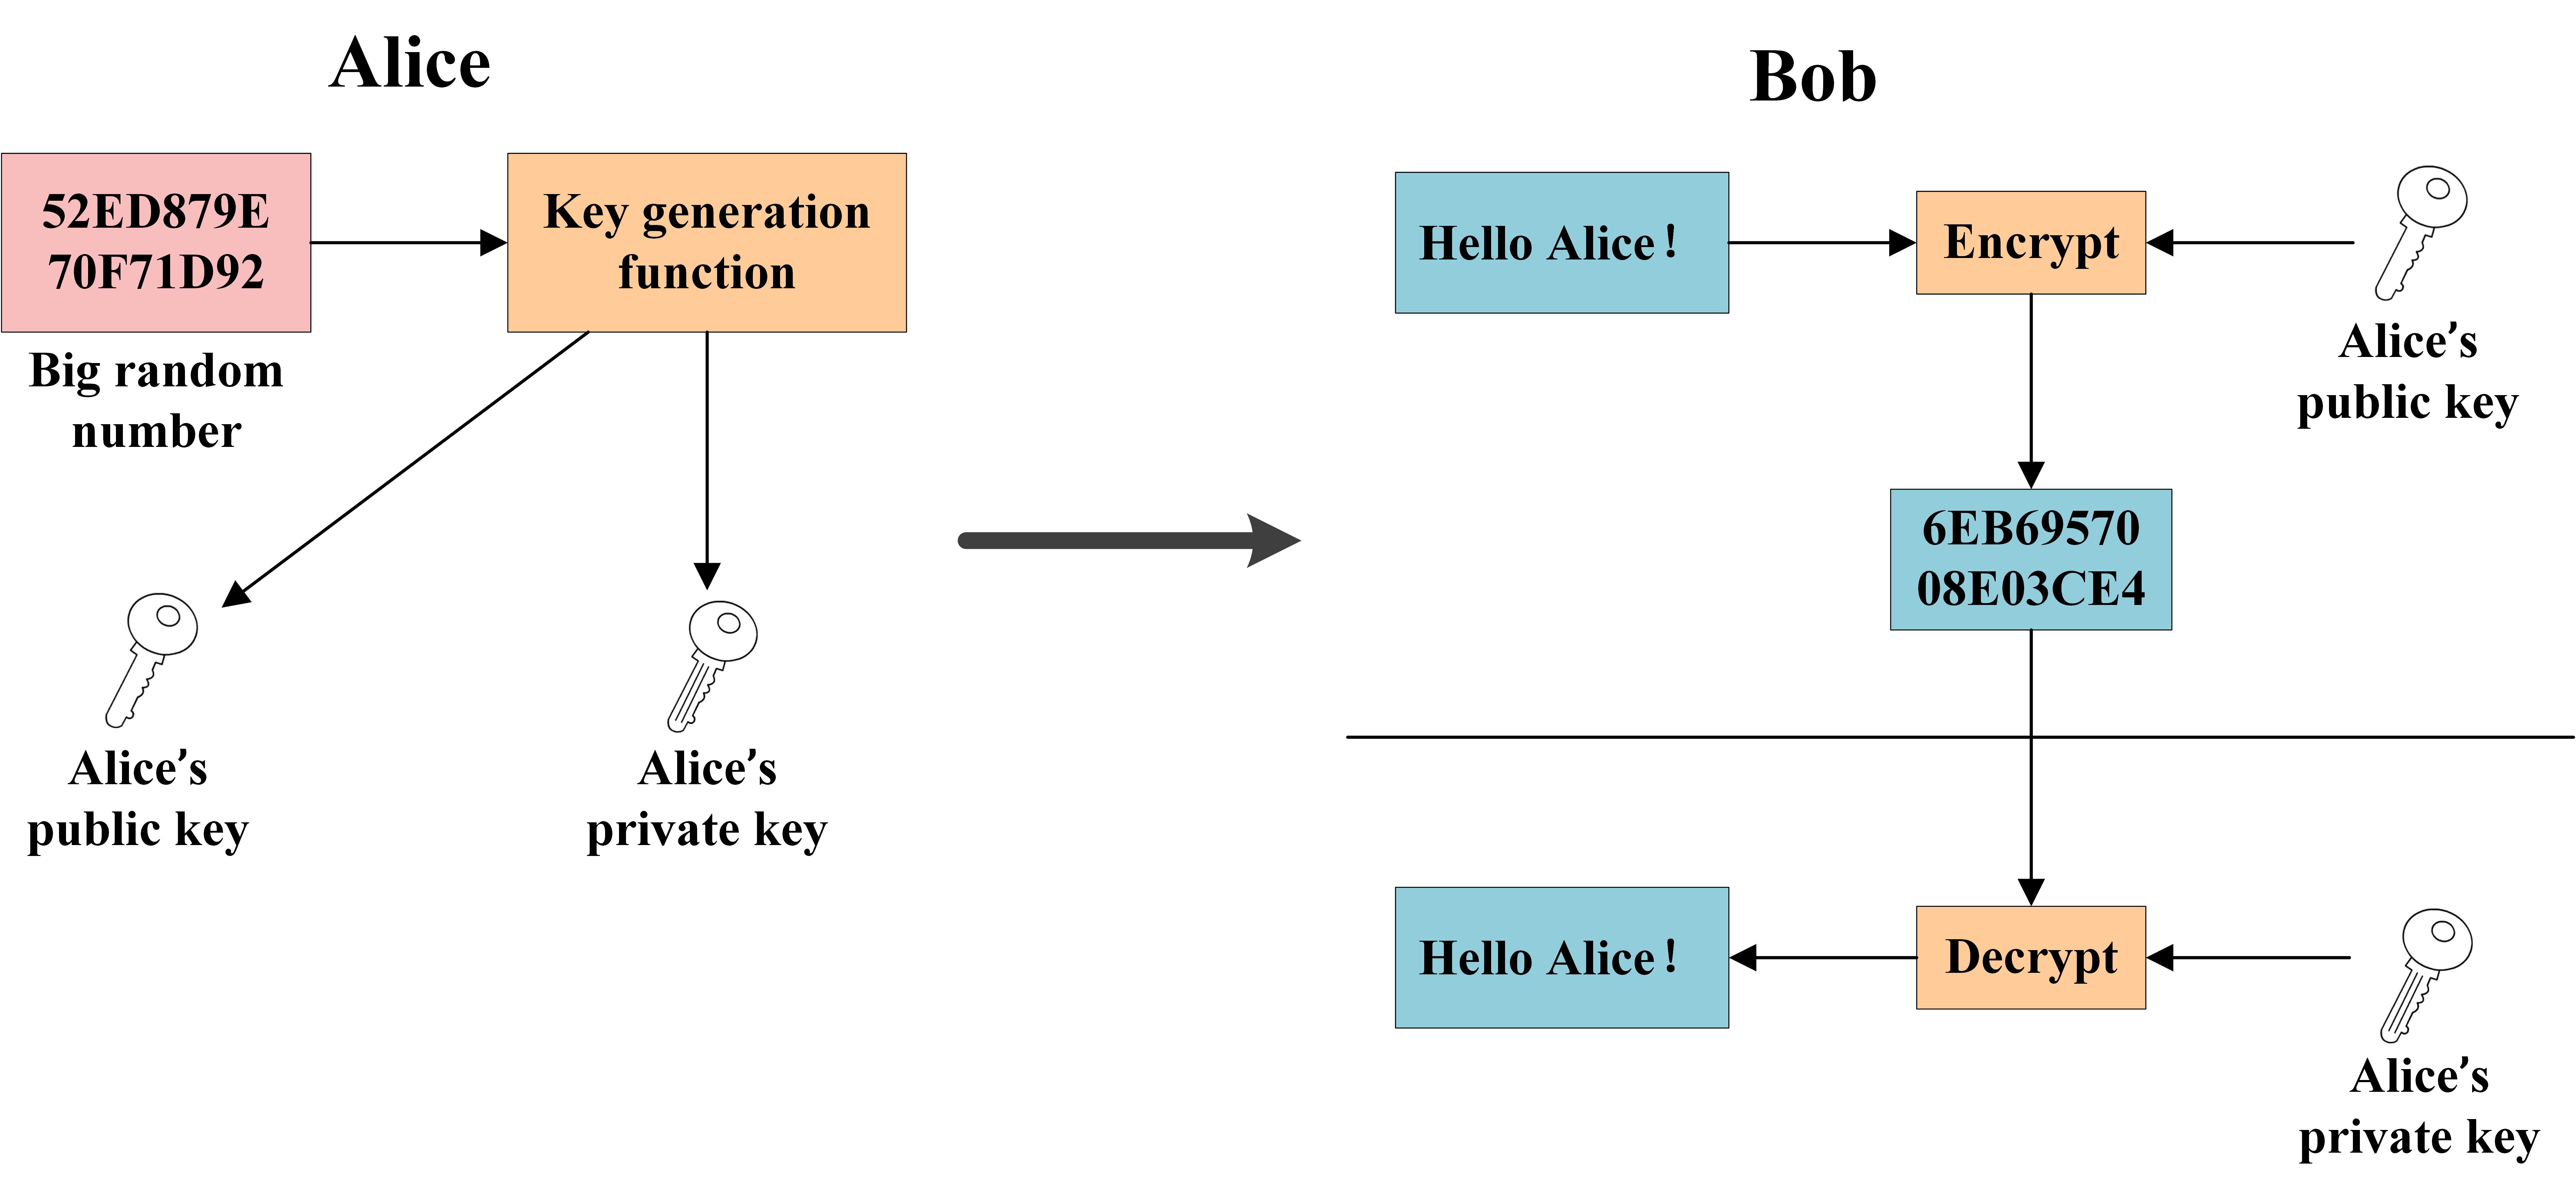
\includegraphics[width=13cm]{figures/pica2.png}
	\caption{典型公钥密码系统}
	\label{pica2}
\end{figure}

在实际使用中,为了平衡对称密码和非对称密码的优缺点,双方之间进行通信通常使用混合加密系统\cite{menezes2018handbook}。首先使用非对称加密在彼此之间达成共享会话密钥(如Diffe-Hellman密钥交换协议),然后使用对称加密传输实际数据。混合加密体制已经安全高效的运行了许多年,但是量子计算的快速发展给以数学问题复杂性为基础的公钥密码体制和以密钥长度为安全基础的对称密码体制带来了灾难性的影响,将使得目前主流的密码体制变得不堪一击\cite{steane1998quantum}。

针对当前密码体制面临的量子计算威胁,近年来美国国家标准与技术研究院(National Institute of Standards and Technology, NIST)已经开始组织设计后量子密码技术(Post-Quantum Cryptography, PQC)\cite{bernstein2009introduction}。后量子密码技术即探索在量子计算条件下的非线性多项式时间可解的 NP 数学问题,典型例子如格基加密算法和基于哈希的加密算法等。无论是经典密码体制,抑或是PQC,其安全性基础都建立在计算资源有限条件下的数学难解问题,无法满足香农提出的信息论安全(Information-theoretical security)级别的信息加密服务。信息论安全通信由信息论安全的密钥分发和信息论安全的加密算法来保证,1949~年,C. E. Shannon 首次系统阐述了消息使用一次一密(One time pad, OTP)算法可以满足无条件安全通信的要求,并指出该算法所使用密钥的熵必须大于等于明文的熵\cite{shannon1949communication}。

物理密码技术的出现打破了传统密码技术的发展瓶颈,并迅速成为国际上信息安全技术的研究热点,以达到信息论防护级别的量子密钥分发(Quantum key distribution, QKD)和物理不可克隆函数(Physical unclonable functions, PUF)为典型代表。量子密钥分发于~1984~年C. H. Bennett和G. Brassard首次提出,基于量子力学的基本特征(不可克隆定理,量子纠缠,测不准原理)为Alice和Bob提供了信息论安全的密钥交换\cite{bb84first,shor2000simple}。因此,Alice和Bob可以基于量子态的传输和测量来共享密钥,而Eve在不引入扰动的情况下无法提取有关密钥的任何信息\cite{gisin2002quantum,liuboliangzi}。量子密钥分发由于其中继转发和经典认证等问题,目前还难以大面积实用化,但是其理论研究和工程实践的成果不仅推动了物理密码的发展,还带来了量子信息领域的变革\cite{xu2020secure,pirandola2020advances,maes2013physically,bennett1992experimental}。物理不可克隆函数最早可追溯至 2001 年 R. Pappu 等人提出的物理单向函数(Physical one-way functions, POF)概念,是一种基于物理、生物微观结构构建 POF 的思想\cite{Pappu2002Physical},并由 B. Gassend 等人实现第一个硅基集成电路 PUF\cite{gassend2002}。PUF 是一种架构在物理实体上的函数关系,挑战响应由其特殊的物理结构决定,并且特定输入对应唯一输出,具备唯一性、稳定性且不可预测,PUF 的不可克隆特性来源于制造(成长)过程中的不可避免的微小偏差\cite{maes2013physically,halak2018physically}。

半导体超晶格密钥分发是基于孪生超晶格 PUF 驱动混沌同步的一种新型信息论安全密钥分发方案,超晶格密钥分发技术是一种物理随机数的异地共享技术拓展。使用孪生超晶格 PUF 物理实体的预分配代替密钥信息的预分配,由器件不可克隆避免了密钥管理中的敏感信息泄露风险;并且,部署完成的孪生超晶格密钥分发设备,能在公开信道中建立密钥分发协议机制,降低密钥部署和更新的成本,以高速、便捷、随遇组网等特点逐渐成为国内研究热点\cite{liu2018secret,wu2020experimental}。


\section{超晶格密钥分发}
\subsection{超晶格研究历史} 
XXXXXXX





\subsection{超晶格物理不可克隆孪生机理}
XXXXXXX


\subsection{基于孪生超晶格的密钥分发方案}

基于超晶格 PUF 的物理不可克隆孪生特性,陈小明等人提出了利用该特性实现点对点密钥分发的构想\cite{chen2020}。超晶格孪生器件在密码学上可以认为是在异地各自运行的同一密钥同一单向函数,且攻击者无法克隆器件也无法建模器件的任意运行过程及结果。因此利用孪生超晶格器件可以安全实现物理随机数的异地排他性共享,即密钥分发\cite{wu2020experimental,xie2021high}。密钥协商的原理架构如图 \ref{pica10} 所示,可简述如下: 
\begin{enumerate}[(1)]
	\item 定义 Alice 为密钥产生(重建)端,Bob 为密钥重建(产生)端,Alice 和 Bob 在常规通信信道上协商激励信号$C$(可以由第三方负责发送,也可由其中一方传给另一方);
	\item Alice 和 Bob 分别在各自的超晶格 PUF 中输入$C$得到原始输出数据,对原始输出进行高精准离线序列同步得到响应$W$和$W'$,$W$和$W'$汉明距离大约为 10\% ;
	\item Alice 计算辅助数据$H$,并将$H$通过公开信道传送给 Bob,Bob 在$H$的帮助下和$W'$计算出$W$,此过程即为信息调同(Information reconciliation)\cite{dodis2004fuzzy};
	\item Alice、Bob 双方根据$H$泄露的信息和器件输出的极小熵,从$W$中提取出相同密钥$R$,此过程即为保密增强(Privacy amplification, PA)\cite{bennett1995generalized}。
\end{enumerate}


\begin{figure}[h]
	\centering
	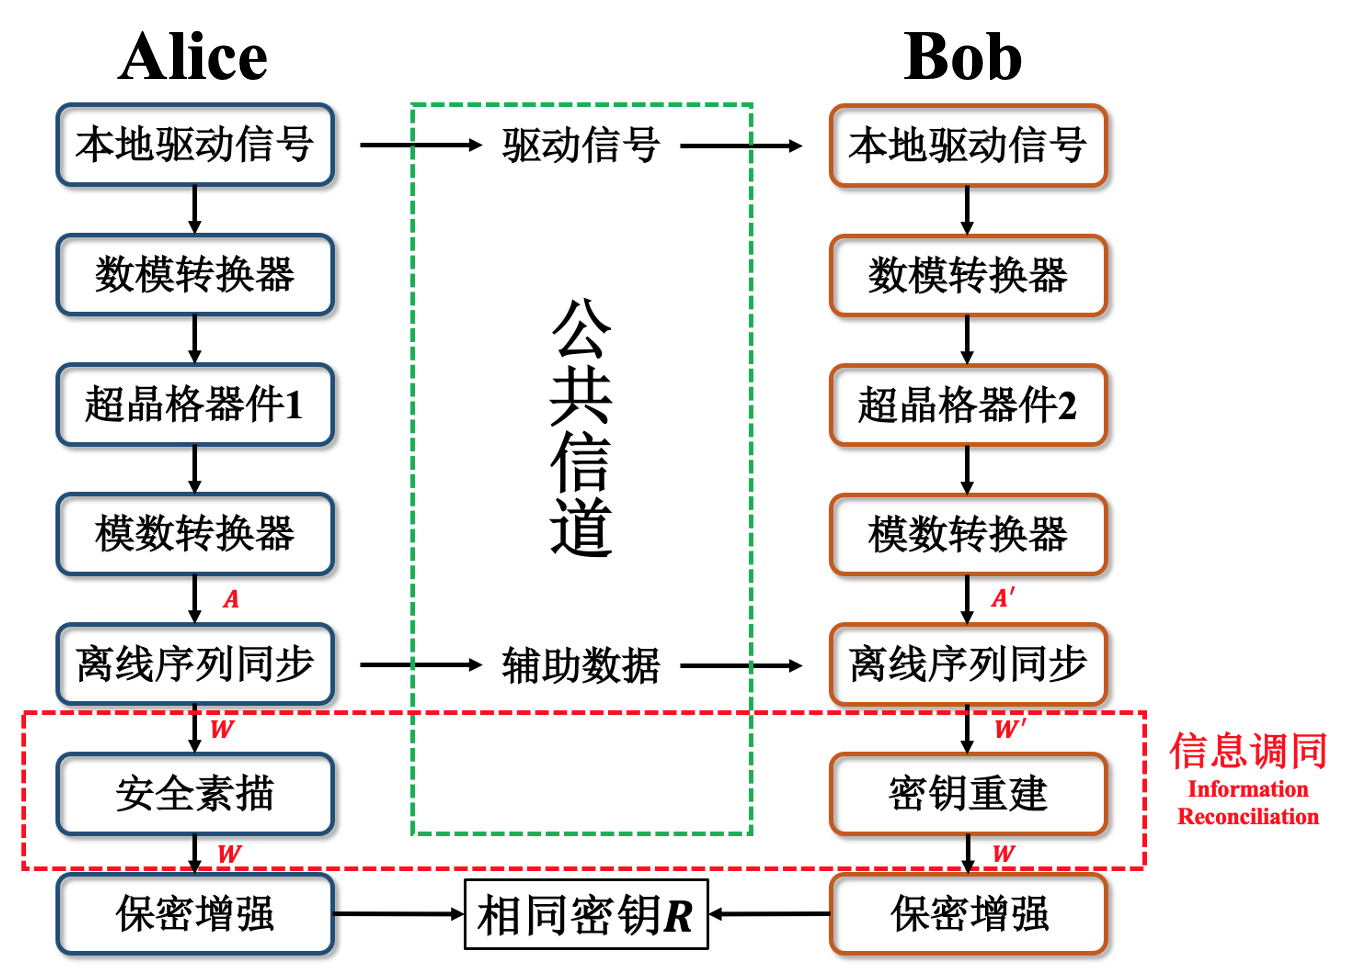
\includegraphics[width=13cm]{pica10.png}
	\caption{基于超晶格PUF的密钥分发协议}
	\label{pica10}
\end{figure}

信息调同用来描述从$W'$恢复出$W$的过程,此过程不会泄漏很多关于$W$的信息,一般用安全素描实现。保密增强的一般实现方案为一致哈希函数(Universal hash functions, UHF)提取器实现\cite{carter1979universal},该函数的输入为非满熵的待提取的随机数和公开的满熵随机数,输出保密的满熵随机数。信息调同和保密增强统称模糊提取器(Fuzzy extractor),可以从物理、生物等唯一特征数据中提取出可用作加密、认证的密钥。


\section{论文主要工作与结构安排}
\subsection{主要工作}

本文的主要研究内容是超晶格密钥分发系统的后处理部分,研究面向实际应用的高精准序列同步算法、高吞吐率的信息调同算法、无条件安全保密增强算法,并开展了相关实验验证。本文对超晶格密钥分发系统的高速高效后处理算法进行了深入研究,取得的主要创新工作如下:

\begin{enumerate}[(1)]
	\item 研究超晶格密钥分发过程中通信双方的高精准序列同步技术。XXXXXXX
	\item 研究高吞吐率的信息调同技术。XXXXXXX
	\item 研究超晶格密钥分发无条件安全保密增强技术。XXXXXXX
	\item 超晶格密钥分发系统安全密钥分发实验。XXXXXXX
\end{enumerate}

\subsection{结构安排}

本文结构组织如下:

第\ref{ch1}章,绪论,即本章。从现代密码学中的密钥管理问题介绍了现今物理密码体系的发展和突破,进而引出超晶格密钥分发技术,介绍了超晶格密钥分发系统后处理技术的研究背景、意义以及本文的主要研究内容。

第\ref{ch2}章,超晶格密钥分发后处理技术基础,主要介绍XX。

第\ref{ch3}章,高精准序列同步技术研究。XXXXXXX。

第\ref{ch4}章,高吞吐率的信息调同算法研究。XXXXXXX

第\ref{ch5}章,信息论安全的保密增强算法研究。XXXXXXX

第\ref{ch6}章,异地实时超晶格密钥分发实验。XXXXXXX

第\ref{ch7}章,总结与展望。对全文工作进行总结,并对未来研究作出展望。



\chapter{超晶格密钥分发后处理算法基础}
\label{ch2}

\emph{\kaishu 合抱之木,生于毫末;九层之台,起于累土;千里之行,始于足下。}

\emph{\kaishu \hfill ---老子}\\


本章介绍了一些基本定义、示例等用于描述基本概念和基础知识。其中包括信息论基础、信道编码基础以及一致哈希函数提取器等相关内容。


\section{熵}


香农于 1948 年在“通信的数学原理”一文中首次将物理热力学中熵的概念引入信息论中,因而迎来信息论学科研究的热点。信息是指某一过程中包含的不确定性,而熵就是用来度量这种不确定性的指标,它反映了在观察一个值之前预测该值的不确定性(熵值)\cite{gray2011entropy}。

\begin{definition}{(\textbf{香农熵,Shannon Entropy}):}
	设随机变量$X$的取值为$x_1,x_2,...,x_n$,与之对应的分布概率为$p_1,p_2,...,p_n$。则$X$的香农熵为
	\begin{equation}
		H(X)=-\sum_{i=1}^{n}p_i\log p_i.
	\end{equation}
\end{definition}



相比较于上述香农熵的讨论,本文更关注Rényi熵。Rényi熵是Alfred Rényi于 1976 年提出的对香农熵、碰撞熵、极小熵的推广。在后文的保密增强算法中,二阶Rényi熵是能从理论上被证明可以提取出无条件安全的密钥,而相关文献也报道了关于利用香农熵提取密钥的安全风险问题。
\begin{definition}{(\textbf{Rényi熵,Rényi Entropy}):}
	设随机变量$X$的取值为$x_1,x_2,...,x_n$,与之对应的概率为$p_1,p_2,...,p_n$。则$X$的Rényi熵为
	\begin{equation}
		H_{\alpha}(X)=\frac{1}{1-\alpha}\log (\sum_{i=1}^{n}p_i^{\alpha}).
	\end{equation}
\end{definition}
当$\alpha=1$时,上式表示 Shannon 熵,当$\alpha=2$时,即二阶Rényi熵,也称作碰撞熵,此时式中的概率表示为碰撞概率$p_c(i)$。但是很多物理系统计算其碰撞熵是相当复杂的,因此目前许多文献都表明计算极小熵用于提取无条件安全的密钥方案是切实可行的。当$\alpha=\infty$时,定义极小熵如下:
\begin{definition}{(\textbf{极小熵,Min-Entropy}):}
	设随机变量$X$的可预测性用$\max_xP[X=x]$表示,那么随机变量$X$的极小熵定义为
	\begin{equation}
		H_{\infty}(X)=-\log(\max_xP[X=x]).
	\end{equation}
\end{definition}
通常情况下,平均极小熵更为准确,因为实际系统中攻击者有各种因素在平均情况下获得与随机变量$X$不独立的事件$Y$。
\begin{definition}{(\textbf{平均极小熵,Average Min-Entropy}):}
	给一对随机变量$X$和$Y$,假如对手知道随机变量$Y$中的$y$,则变量$X$的可预测性用$\max_x P[X=x|Y=y]$表示, 所以对手以$E_{y\leftarrow Y}(\max_x P[X=x|Y=y])$预测$X$,那么变量$X$的平均极小熵定义为
	\begin{equation}
		\tilde{H}_{\infty}(X|Y)=-\log(E_{y\leftarrow Y}(\max_x P[X=x|Y=y]))=-\log(E_{y\leftarrow Y}(2^{-H_{\infty}(X|Y=y)})).
	\end{equation}
\end{definition}


\section{信道编码基础}
\subsection{纠错码介绍}
基于上述互信息量的介绍,我们可以分析有噪信道下的信息保真传输问题,即香农第二定理,有噪信道编码定理,设信道的输入为$X$,输出为$Y$,首先定义信道容量为$C=\max_{P(X)}I(X;Y)$。
\begin{theorem}{(\textbf{有噪信道编码定理,Noisy channel coding theorem}):}
	每个信道都有自己对应的信道容量$C$,当信息编码码率$R\leq C$且码长足够长的情况下,总可以找到一个码字,可以使用最大似然译码,使得误码率随着码长$N$的增加而减小至趋于0。
\end{theorem}
香农提出有噪信道编码定理之后,各种纠错码实现方案如雨后竹笋般出现\cite{zhuxue2001},追求香农为我们设定的天花板。


XXXX。

\subsection{信道模型}
用$\mathcal{X}$表示信道输入,$\mathcal{Y}$表示信道输出。对于离散信道模型\cite{lin2001error},我们用离散概率$Pr_{Y|X}(y|x)$描述随机变量$X$和$Y$的信道模型。对于连续信道模型,我们用条件密度$f_{Y|X}(y|x)$表示。如果$|\mathcal{X}|=2$表示二元输入信道,即$\mathcal{X}=\{-1,+1\}$或$\mathcal{X}=\{0,1\}$。

\begin{definition}{(\textbf{二元擦除信道,Binary erasure channel, BEC}):}
	参数为$\epsilon$的二元擦除信道表示为$BEC(\epsilon)$。信道输入端的随机变量$X$可以取值$x\in X=\{-1,+1\}$,信道输出端的随机变量$Y$可以取值$y\in Y=\{-1,?,+1\}$。转移概率表示如下:
	
	\begin{equation}
		Pr_{Y|X}(y|x)=\left\{
		\begin{array}{rcl}
			1-\epsilon,       &      & {y=x,}\\
			\epsilon,     &      & {y=?,}\\
			0,     &      & {otherwise}
		\end{array} \right.
	\end{equation}
	
\end{definition}


XXX。

\subsection{BCH码}
XXXX。

\subsection{LDPC码}
低密度奇偶校验(Low-density parity-check, LDPC)码是由 Gallager 于 1963 年提出\cite{gallager1962low},并且证明了 LDPC 码的性能接近信道容量且非常易于实现。但是 LDPC 码在当时由于计算机计算能力受限和存储较小等问题导致当时的人们认为该码是不符合实际的(impractical)。在上世纪 90 年代由于计算机存储和计算技术的蓬勃发展,LDPC 码被 MacKay,Luby 等人重新提出,从而进入研究的热点,并很快成为深空通信,移动通信,卫星通信等信道编码标准\cite{ryan2009channel}。

XXXX。


\subsection{Polar码}
Polar 码一种基于信道极化理论的线性分组码,由土耳其 Bilkent 大学教授 Erdal Arikan 于 2007 年提出\cite{arikan2011systematic},应用 Polar 码时,首先选定码长$n$和信息位长度$k$,然后需要对所选的信道进行极化,此时可以确定 Polar 码放入编译码结构。Polar 码的编码过程和 BCH 码等代数编码思想一致,译码过程采用串行抵消译码算法,时间复杂度为$O(n\log n)$。Polar 码是目前唯一被证明在$n\rightarrow \infty$时、利用串行抵消译码算法性能达到香农限的纠错码。


XXXX。


\section{提取器基础知识}
\subsection{强提取器和统计距离}

随机性提取也叫做提取器,是指从弱安全的原始随机序列提取出与均匀分布统计距离可忽略的无条件安全随机数的函数。提取器自提出之后便得到广泛研究,无论是在密码学上还是计算机中的分布式计算都实现了大规模应用,尤其在物理随机数发生器的后处理过程。由于弱提取器的密钥不可公开导致无法开展实际应用,本文叙述的提取器若不具体说明均为强提取器。首先定义两个分布的统计距离如下:

\begin{definition}{(\textbf{统计距离,Statistical Distance}):}
	设$X$和$Y$是集合$\mathcal{M}$上的两个随机变量,$X$和$Y$之间的统计距离定义为:
	\begin{equation}
		\mathbf{SD}(X,Y)=\frac{1}{2}\sum_{\omega}|Pr[X=\omega]-Pr[Y=\omega]|.
	\end{equation}
\end{definition}
如果$X$和$Y$之间的统计距离$\mathbf{SD}(X,Y)\leq \epsilon$,则称$X$和$Y$是$\epsilon$统计接近的,如果$\epsilon$是可忽略的,则称$X$和$Y$是统计不可区分的。如果对于提取出的随机数与均匀分布的统计距离$\epsilon$是可忽略的,那么即可认为提取器输出的随机数是可用的。

\begin{definition}{(\textbf{强提取器,Strong Extractor}):}
	对于式子$Ext:\{0,1\}^n \times \{0,1\}^r\ \rightarrow \{0,1\}^l$,如果对于所有的最小熵为$m$的分布$W$,有
	\begin{equation}
		\mathbf{SD}((Ext(W;X),X),(U_l,X)) \leq \epsilon,
	\end{equation}
	其中$X$是$\{0,1\}^r$上的均匀分布,$U_l$表示$l$比特的均匀分布的随机数,则$Ext$是一个$(n,m,l,\epsilon)$强提取器
	
\end{definition}


\subsection{一致哈希函数}
经典密码学中的哈希函数通常具有单向性、雪崩性等特点,可作为提取器使用,但是单个哈希函数对于所有的输入无法满足提取器的要求。一致哈希函数簇是一族哈希函数的统称,每次均匀的从一族哈希函数中选择一个应用于待提取样本。








\section{本章小结}
本章介绍了超晶格密钥分发后处理技术的相关基础知识,包括信息论基础,信道编码基础,提取器相关内容介绍,这部分内容为信息调同、保密增强等后处理技术打下了坚实的基础。XX。



\chapter{后处理方案改进及高精准序列同步算法研究}
\label{ch3}
\emph{\kaishu 昨夜西风凋碧树,独上高楼,望尽天涯路。}

\emph{\kaishu \hfill ---晏殊}\\

超晶格密钥分发过程中通信双方得到一致的驱动序列后,激励孪生超晶格产生相似的原始数字序列。


\section{在线序列同步技术}
\subsection{原理方案}
XXXX。





\subsection{实验结果与分析}

XXXXXXXX。

\section{高精准离线序列同步技术}

\subsection{原理方案}
由于在线同步算法的计算复杂度和通信负载在实际应用中难以接受,因此本文设计了一种追峰算法来进行超晶格输出序列的高精准同步,无需进行通信交互。

XXXX。

\subsection{实验结果与分析}

XXXX。




\section{超晶格密钥分发协议实现方案改进}

XXXXX。

\section{本章小结}
本章首先研究了在线同步算法在超晶格 PUF 激励响应的序列同步问题的应用,并进行了相关实验评估了在线同步算法的准确性、效率、资源消耗等。


\chapter{高吞吐率的信息调同算法研究}
\label{ch4}

\emph{\kaishu 衣带渐宽终不悔,为伊消得人憔悴。}

\emph{\kaishu \hfill ---柳永}\\

经过高精准离线序列同步后,Alice 和 Bob 间的比特串由于模拟系统不可避免的差异仍然有不一致的地方,所以需要通过信息调同技术使两边的比特序列达成一致。

\section{信息调同问题模型}
信息调同问题最早由 Bennett 提出并应用于量子密钥分发\cite{bennett1992experimental},随
后 Brassard 提出信息调同的公开讨论模型使其正式步入实用化\cite{brassard1993secret}。



\begin{definition}{(\textbf{信息调同的信道编码等效模型,Equivalent model of information reconciliation as channel coding}):}
	$\mathcal{M}$是具有距离函数$dis$的度量空间(Metric Space),一个参数为$(\mathcal{M},m,\tilde{m},t)$的信息调同算法分为“产生”(GEN)和“重建”(REC)两个阶段,具有如下三个性质:
	\begin{itemize}
		\item 在产生阶段,输入$w\in \mathcal{M}$,输出辅助数据$GEN(w)=h\in \{0,1\}^*$;
		\item 在重建阶段,输入$w' \in \mathcal{M}$和产生阶段输出的辅助数据$h$,在保证$dis(w,w')\leq t$的前提下,能够得到$REC(w',h)=w$;
		\item 安全性保障:对$\mathcal{M}$上的任意分布$W$都有极小熵$m$,$W$的值可以被第三方通过观察辅助数据$s$获得的信息不超过$2^{-\tilde{m}}$,即$\tilde{H}_{\infty}(W|h)\geq \tilde{m}$。
	\end{itemize}
\end{definition}


XXXXX。

\section{基于BCH码的高速纠错方案}
\subsection{编译码方案}
BCH 码是一种典型的线性分组码,在码长较短时具有出色的性能表现。他的结构简单,易于实现,在资源受限的场景下很受欢迎。因此目前常见的PUF认证系统以及大多数 SSD 控制器大多采用 BCH 码作为其纠错方案。BCH 码在码长 $n$ ,信息位长度 $k$ ,和纠错能力 $t$ 之间存在严格的代数关系。对于任何的正整数 $m \geq 3$并且$t<2^{(m-1)}$ ,都会存在一个如式 (\ref{eq4-1}) 所示参数的一个二元 BCH 码。



\begin{equation}
	\left\{
	\begin{split}
		n=2^m-1 \\
		n-k \leq mt \\
		d_{min}\geq 2t+1
	\end{split}
	\right.
	\label{eq4-1}
\end{equation}


\begin{algorithm}[H]
	\KwData{$R(x)$, $LT$, $ALT$, $blockNum$}
	\KwResult{译码码字$C$}
	Initialize parameters, $\sigma^{(0)}(x)=1$, $D(0)=0$, $d_0=s_1$, $\sigma^{(-\frac{1}{2})}(x)=1$, $D(-\frac{1}{2})=0$, $d_{-\frac{1}{2}}=1$\;
	$\#$pragma omp parallel for shared($LT$, $ALT$) firstprivate($R(x)$)\;
	threadNum = 0\;
	\While{threadNum < $blockNum$}{
		计算 syndrome polynomial $S=\{s_1,s_2,\cdots,s_{2t}\}=\{R(\alpha),R(\alpha^2),\cdots,R(\alpha^{2t-1})\}$\;
		从BM算法计算错误位置多项式\;
		\While{$j < 2t$}{
			\If {$d_j==0$}{
				$\sigma^{j+1}(x)=\sigma^{j}(x)$\;
				$D(j+1)=D(j)$\;
			}
			\Else {
				计算$d_{j+1}$\;
				$\sigma^{j+1}(x)=\sigma^{j}(x)-d_jd_i^{-1}x^{j-i}\sigma^{i}(x)$\;
			}
			一直迭代直到计算出$\sigma^{t}(x)$\;	    
		}
		从Chien搜索算法计算$\sigma(x)$的根,根取反即错误位置\;	
		threadNum = threadNum + 1\;
	}
	The output is codeword $C$\;
	\caption{优化后的BCH码译码器}
	\label{alg4-1}
\end{algorithm}

XXXXXX。

\subsection{实验结果与分析}

本文在室温实验室环境下采集孪生超晶格 PUF 的输出,通过高精准序列同步算法后量化为二元序列,并按照码长$n=4095$进行分组总共得到 120,000 组数据。


XXXXX。

\section{基于LDPC码的高速纠错方案}

在上一节中我们提出了基于BCH码的超晶格信息调同高速纠错方案,但是BCH码在码长较长时性能表现一般,速度差强人意,无法满足更高速率的超晶格密钥分发系统的需求,因此需要更高效的纠错方案来加快系统吞吐率。

\subsection{编译码方案}
1963 年,Robert G. Gallager 的博士论文中论述了校验矩阵为稀疏矩阵的纠错码,进而创新性的提出一种新的线性分组码,LDPC 码。刚开始提出由于当时计算机的计算性能的限制和理论研究的现状导致当时被认为是不符合实际的,使其无法得到长足发展。MacKay,Luby 在上世纪 90 年代重新将 LDPC 码进一步发展\cite{mackay1996near},随着计算机存储和计算性能的逐渐发展 LDPC 码逐渐成为研究热点方向,在目前计算机的高速发展的今天,LDPC 码以其在各种信道上提供接近香农限的性能立足在各大传输和存储设备的纠错编码的应用上。

XXXXXX。


\subsection{实验结果与分析}

同上一节BCH码优化方案测试吞吐率使用相同的超晶格数据,对于设计的这四种LDPC码,按照码长进行分组我们同样测试了 120,000 组码字数据。

XXXXX。

\section{基于Polar码的高速纠错方案}

Polar 码是一种由信道极化理论演化而来的新型线性分组纠错码,于 2007 年被 Arikan 提出。Polar 码由于其优异的性能一经提出便受到广泛关注,对于超晶格密钥分发系统也是如此,Polar 码的诸多特性使其对超晶格密钥分发系统的纠错方案极其匹配。首先,Polar 码是第一个在理论上被证明可以达到香农限的纠错码,是一类具有较低的编码和译码复杂度的纠错码,尤其在码长较长时表现优异。再者,和LDPC码不同的是,Polar 码和 BCH 码一样容易构造,只要确定了码长和码率其结构就可以确定。此外,Polar 码的另外一个重要特点是其译码器的规则递归结构,使得译码器的软件实现速度大大高于其他纠错码\cite{mori2009performance}。

\subsection{编译码方案}

XXXXX。



\subsection{实验结果与分析}



XXXX。


\section{分析比较}

XXXX。




\section{本章小结}
在本章中,我们提出了一种针对超晶格密钥分发系统的多线程高吞吐率的信息调同纠错方案,本文提出的纠错优化方案可以高效地应用于不同的场景。XXXX。
\chapter{信息论安全的保密增强算法研究}
\label{ch5}

\emph{\kaishu 众里寻他千百度,蓦然回首,那人却在,灯火阑珊处。}

\emph{\kaishu \hfill ---辛弃疾}\\

保密增强是超晶格密钥分发系统实现安全密钥提取的至关重要的步骤,其目标是剔除超晶格原始输出不足熵以及后处理过程中攻击者可能获取的部分密钥串信息,并生成相对于攻击者而言信息论安全的密钥。

\section{保密增强问题模型}

XXXXXX。


\section{极小熵评估}
\subsection{定义和假设}


XXXXXX。


\subsection{基于超晶格PUF的随机模型}

XXXXXXXXX。


\subsection{极小熵结果与分析}

在本节中,我们在室温实验室环境下采集多组超晶格PUF的原始输出数据,对提出的极小熵估计算法进行了多组实验以得到准确的评估结果。



$$P=\begin{bmatrix}  
	0.088235 & 0.058824 & 0.147059 & 0.147059 & 0.235294 & 0.117647 & 0.029412 & 0.176471 \\
	0.205882 & 0.088235 & 0.235294 & 0.000000 & 0.058824 & 0.205882 & 0.088235 & 0.117647 \\
	0.073171 & 0.170732 & 0.170732 & 0.146341 & 0.048780 & 0.073171 & 0.170732 & 0.146341 \\ 
	0.147059 & 0.088235 & 0.147059 & 0.117647 & 0.117647 & 0.147059 & 0.117647 & 0.117647 \\
	0.113636 & 0.090909 & 0.113636 & 0.113636 & 0.295455 & 0.068182 & 0.136364 & 0.068182 \\
	0.114286 & 0.085714 & 0.142857 & 0.171429 & 0.057143 & 0.085714 & 0.257143 & 0.085714 \\
	0.078947 & 0.184211 & 0.078947 & 0.131579 & 0.157895 & 0.052632 & 0.131579 & 0.184211 \\
	0.102564 & 0.128205 & 0.102564 & 0.076923 & 0.179487 & 0.205128 & 0.076923 & 0.128205 \\
\end{bmatrix}$$




\section{保密增强算法实现方案}
\subsection{输出密钥长度估算}

XXXXXX。

\begin{theorem}
	假设函数簇$\{H_x:\{0,1\}^n\rightarrow \{0,1\}^l \}_{x\in X}$是一致哈希函数簇,信息调同过程的纠错码为$(n,k,t)$,任意随机输入$W$的极小熵为$m$,那么$l\leq m-(n-k)-2\log \frac{1}{\epsilon}+2$。
\end{theorem}



\begin{proof}
	首先由剩余哈希引理可知,对任意的随机输入$W$,有
	\begin{equation}
		SD((H_x(W),X),(U_l,X)) \leq \frac{1}{2\sqrt{2^{-H_{\infty}(W)+l}}},
		\label{eq5-12}
	\end{equation}
	其中,$U_l$表示$\{0,1\}^l$上的均匀分布。又$\frac{1}{2\sqrt{2^{-H_{\infty}(W)+l}}} \leq \epsilon$可知
	\begin{equation}
		l\leq m-2\log\frac{1}{\epsilon}+2,
		\label{eq5-13}
	\end{equation}
	其中$m$表示平均条件下的$W$的极小熵,上述定理说明保密增强的熵损失为$2\log \frac{1}{\epsilon}-2$的比特数,即最多能够提取出$m-2\log \frac{1}{\epsilon}+2$长度的满熵比特。
	
	下面再证明信息调同过程中的熵损失为$(n-k)$即可。首先给出一个引理以便后续证明需要。
	\begin{lemma}
		假设$A,B,C$是随机变量,此时如果$B$至多有$2^{\lambda}$种可能的值,那么
		\begin{equation}
			\hat{H}_{\infty}(A|(B,C))\geq \hat{H}_{\infty}((A,B)|C)-\lambda \geq \hat{H}_{\infty}(A|C)-\lambda,
			\label{eq5-14}
		\end{equation}
		特别的,
		\begin{equation}
			\hat{H}_{\infty}(A|B)\geq \hat{H}_{\infty}(A|B)-\lambda \geq H_{\infty}(A)-\lambda.
			\label{eq5-15}
		\end{equation}
	\end{lemma}
	
	因此,如果公开的helper data至多有$2^{\lambda}$种可能的值,对于任意的信息调同的输入$W$,都有
	\begin{equation}
		\hat{H}_{\infty}(W|hd)\geq  H_{\infty}(W)-\lambda.
		\label{eq5-16}
	\end{equation}
	即表明熵损失最多为$\lambda$。已知$n$表示纠错码码长,$k$表示纠错码的信息位的长度,helper data的长度也为$n$。
	
	那么由上述引理可知,
	\begin{equation}
		\hat{H}_{\infty}(W|(hd,I))\geq \hat{H}_{\infty}((W,hd)|I)-n,
		\label{eq5-17}
	\end{equation}
	又因,
	\begin{equation}
		P(W=w,hd=s|I=i)\leq \frac{1}{2^{k}}P(W=w|I=i).
		\label{eq5-18}
	\end{equation}
	利用式 (\ref{eq5-18}) 可得,
	\begin{equation}
		\hat{H}_{\infty}((W,hd)|I) \geq \hat{H}_{\infty}(W|I)+k,
		\label{eq5-19}
	\end{equation}
	结合式 (\ref{eq5-17}) 和 式 (\ref{eq5-19}) 可知,
	\begin{equation}
		\hat{H}_{\infty}(W|(hd,I))\geq \hat{H}_{\infty}(W|I)+k-n.
		\label{eq5-20}
	\end{equation}
	
	所以,信息调同过程的熵损失为$(n-k)$。
\end{proof}

综上所述,超晶格密钥分发系统最终可提取出的密钥长度为$l\leq m-(n-k)-2\log \frac{1}{\epsilon}+2$,提取出的密钥是满熵的,且该协议过程无条件安全。


\subsection{LFSR-Toeplitz提取器}

XXXXXX。


\subsection{基于FFT的加速方案}

XXXXXX。

\subsection{实验结果}

XXXXXX。




\section{本章小结}
本章给出了


\chapter{异地实时超晶格密钥分发实验}
\label{ch6}

\emph{\kaishu Stay Hungry, Stay Foolish.}

\emph{\kaishu \hfill ---Steve Jobs}\\

XXX


\section{系统架构}

XXXXXXXXXX。


\section{分模块}
\subsection{驱动层}

XXXXXX。

\subsection{功能组件层}

XXXXXX。


\subsection{业务逻辑层}

XXXXXXXXX。


\section{北京--长沙异地实时超晶格密钥分发实验}

XXXXXXXXXXXXX。




\section{本章小结}
本章首先叙述了


\chapter{全文总结与展望}
\label{ch7}

\emph{\kaishu 每个人都会经过这个阶段,见到一座山,就想知道山后面是什么。我很想告诉他,可能翻过去,你会发觉没什么特别,再翻过来,会觉得这边更好。但我知道他不会听,自己不走一走,又怎么会甘心。}

\emph{\kaishu \hfill ---《东邪西毒》}\\

\section{全文总结}

XXXX。本文首先建立了超晶格密钥分发后处理整体架构,分别对序列同步、信息调同、保密增强三个部分的内容展开了研究。本文专注于核心问题展开理论研究和应用拓展,取得的主要研究成果包括:

\begin{enumerate}[(1)]
	\item XXX
	\item XXX
	\item XXX
	\item XXX
\end{enumerate}



\section{后续工作展望}
随着超晶格密钥分发技术实用化的稳步推进,后处理阶段要研究的东西还有很多,尽管作者尽了最大努力进行了本课题的研究,但所做的工作仍然有许多不足,一些研究内容仍需要完善,并且还有如下方向值得进一步探索:

\begin{enumerate}[(1)]
	\item XXX
	\item XXX
\end{enumerate}
\BESTIbackmatter{\bibliography{bib/tex}}

\begin{thanks}


\emph{\kaishu 全情投入,守正出奇,愿等花开。}

\emph{\kaishu \hfill ---佚名}\\

当论文写作接近尾声时,暑天已过去大半,可南方的燥热依旧不减。所幸住在湖边不远,偶尔湖风吹过,又颇有一点“明月别枝惊鹊,清风半夜鸣蝉”之感。回想起这近二十载求学生涯,如梦一场,恍如昨日。时光里有少年的不羁和浪荡,有青春的颓废和迷茫,也有成熟之后的坦然和温暖,白驹过隙,事实上想来,只是寥寥数语。

此刻最为感激的当数硕士生涯为我执灯的恩师陈小明先生。






\end{thanks}


\begin{resume}

\section*{1.\hspace{0.75em}基本情况}
男,安徽XX人,~~XXXX年~X~月出生,北京电子科技学院密码系网络空间安全专业~2019~级硕士研究生。
\section*{2.\hspace{0.75em}教育背景}
\begin{resumelist*}
\resumelistitem 2015.09~~2019.06,XXXXXX,本科,专业:XXXXXX
\resumelistitem 2019.09~\hspace{3.5em},北京电子科技学院,硕士研究生,专业:网络空间安全
\end{resumelist*}

\section*{3.\hspace{0.75em}攻读硕士学位期间的研究成果}
\begin{resumelist}{\hspace{-0.25em}3.1\hspace{0.5em} 发表学术论文}
\resumelistitem \textbf{Zhang san.} et al. XXXXXX. PKC, (2021). 
\end{resumelist}

\begin{resumelist}{\hspace{-0.25em}3.2\hspace{0.5em} 申请(授权)专利}
\resumelistitem 无
\end{resumelist}

\begin{resumelist}{\hspace{-0.25em}3.3\hspace{0.5em} 参与科研项目及获奖}
\resumelistitem 无
\end{resumelist}
\end{resume}

\end{document}
